\definecolor{monVert}{RGB}{120,212,144}
%\tikzstyle{erlang} = [draw, fill=sectionColor, rectangle, minimum height=2em, minimum width=3em]
\tikzstyle{erlang} = [draw, fill=blue!20, rectangle, minimum height=2em, minimum width=3em]
%\tikzstyle{erlang_2} = [draw, fill=green!20, rectangle, minimum height=2em, minimum width=3em]
\tikzstyle{erlang_2} = [draw, fill=monVert, rectangle, minimum height=2em, minimum width=3em]
%\tikzstyle{expo} = [draw, fill=sectionColor, circle,minimum height=2em]
\tikzstyle{expo} = [draw, fill=blue!20, circle,minimum height=2em]
%\tikzstyle{expo_2} = [draw, fill=green!20, circle,minimum height=2em]
\tikzstyle{output} = [coordinate]
\tikzstyle{expo_2} = [draw, fill=monVert, circle,minimum height=2em]



\chapter{Reinfection as a potential phenomenon for influenza pandemics: Tristan da Cunha 1971 epidemic as a case study}


Anton Camacho;
Sébastien Ballesteros;
Bernard Cazelles 


\section{Introduction}

A swine-origin influenza A(H1N1) virus is responsible for the current
pandemic and reminds us that the risk of influenza pandemic is high
and will persist in the future. The lessons from the past are
therefore precious and may help us to anticipate and manage such
disasters. In this context the multiple-wave outbreaks of influenza
type A over one season, which have been reported during several
pandemic episodes of the past century, remain poorly understood. The
most striking example remains the ``Spanish'' influenza pandemic of
1918-1919 that occurred in three waves over 9 months, causing about 50
million deaths worldwide. As a result, successive attacks were
explicitly reported with individuals having experienced up to two
reinfection episodes over a short time interval
\citep{Health1920,Dudley1926,Mantle1973,Barry2008}.

Determining whether these multiple-wave epidemics were caused by the
same strain remains a challenge since there is few or even no virus
samples from each wave. However it is commonly believed that
apparition of new antigenically drifted variants escaping population
immunity takes years, which is inconsistent with the inter-wave
periods of few weeks \citep{Taubenberger2006}.

Although there is a lack of virological and serological analysis of
these epidemiological phenomena, mathematical models can provide
important insight into the underlying mechanisms that could explain
multiple-wave epidemics. These dynamics have been reproduced within
the simple epidemiological $SIR$ (Susceptible-Infectious-Removed)
framework by supposing that coinfection with other acute respiratory
infections increases the transmissibility of influenza virus
\citep{Merler2008} or by altering the structure of the network of
contacts in the course of the epidemic as a defensive behavioral
response \citep{Poletti2009}. However these models cannot explain
cases of multiple infections in the same host during a single epidemic
season. In contrast, \citet{Mathews2007} have introduced a flexible
model that allows for reinfection: following recovery from infection
hosts acquire protective immunity with a certain probability,
otherwise they become again susceptible. From its side,
\citet{Gomes2004} have invoked a partial immune protection for
explaining reinfection. Both mechanisms challenge the common
assumption that infection by an influenza strain confers life-long
protection against reinfection by the same strain \citep{Earn2002}.
Thus, explaining these epidemiological phenomena is not only of public
health policies interest but may also provide a better understanding
of the human immune response to a novel influenza virus.

In this work, we propose to disentangle between three different
biological mechanisms for explaining a two-wave influenza epidemic
with explicit cases of reinfection that occurred on the remote island
of Tristan da Cunha in 1971 and that was reported by
\citet{Mantle1973} (see also Figure \ref{fig:tdc}). This case is all
the more interesting that the small population remained fully isolated
all along the epidemic, ruling out the hypothesis of a second
influenza virus introduction from outside, and that serological
analysis confirmed the presence of influenza type A/H3N2 during both
waves \citep{Mantle1973}.

The emergence of new influenza strains will continue to pose
challenges to public health and to the scientific community. No one
can accurately predict the timing and severity of the next pandemic,
numerous key questions still remain unanswered. The influence of
multiple infections in a naive population is one of the uncertainties
that are critical for improving our understanding and for correctly
describing a given pandemic. Our approach is based on the analysis of
the shape and the timing of observed incidence time series in order to
compare stochastic models constructed with different
assumptions. Identification and comparison of models are achieved
through two recent plug-and-play frameworks perfectly adapted to
nonlinear stochastic models \citep{Ionides2006,Toni2009}. These
frameworks are based on the frequentist \citep{Ionides2006} or on the
bayesian \citep{Toni2009} philosophy and both allow for parameter
inference and model selection.

\begin{figure}
\begin{center}
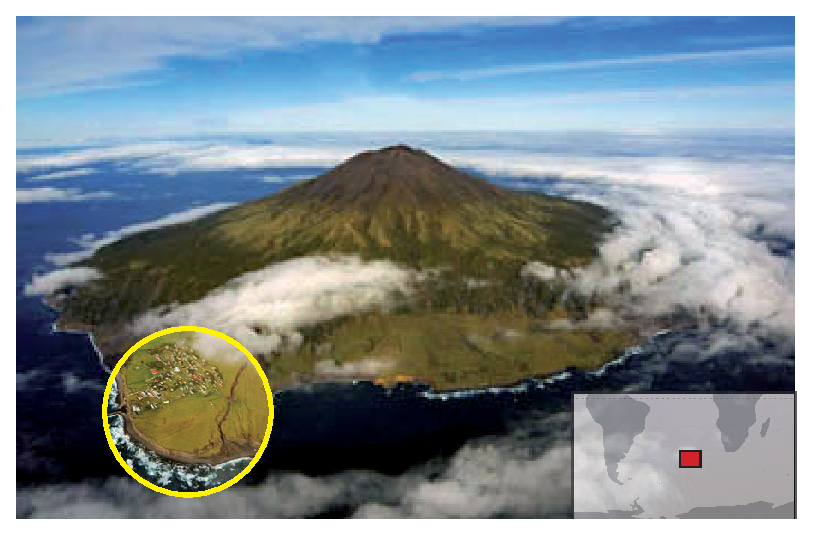
\includegraphics[width=0.7\linewidth]{texte/tdc/graph/tdc.eps}
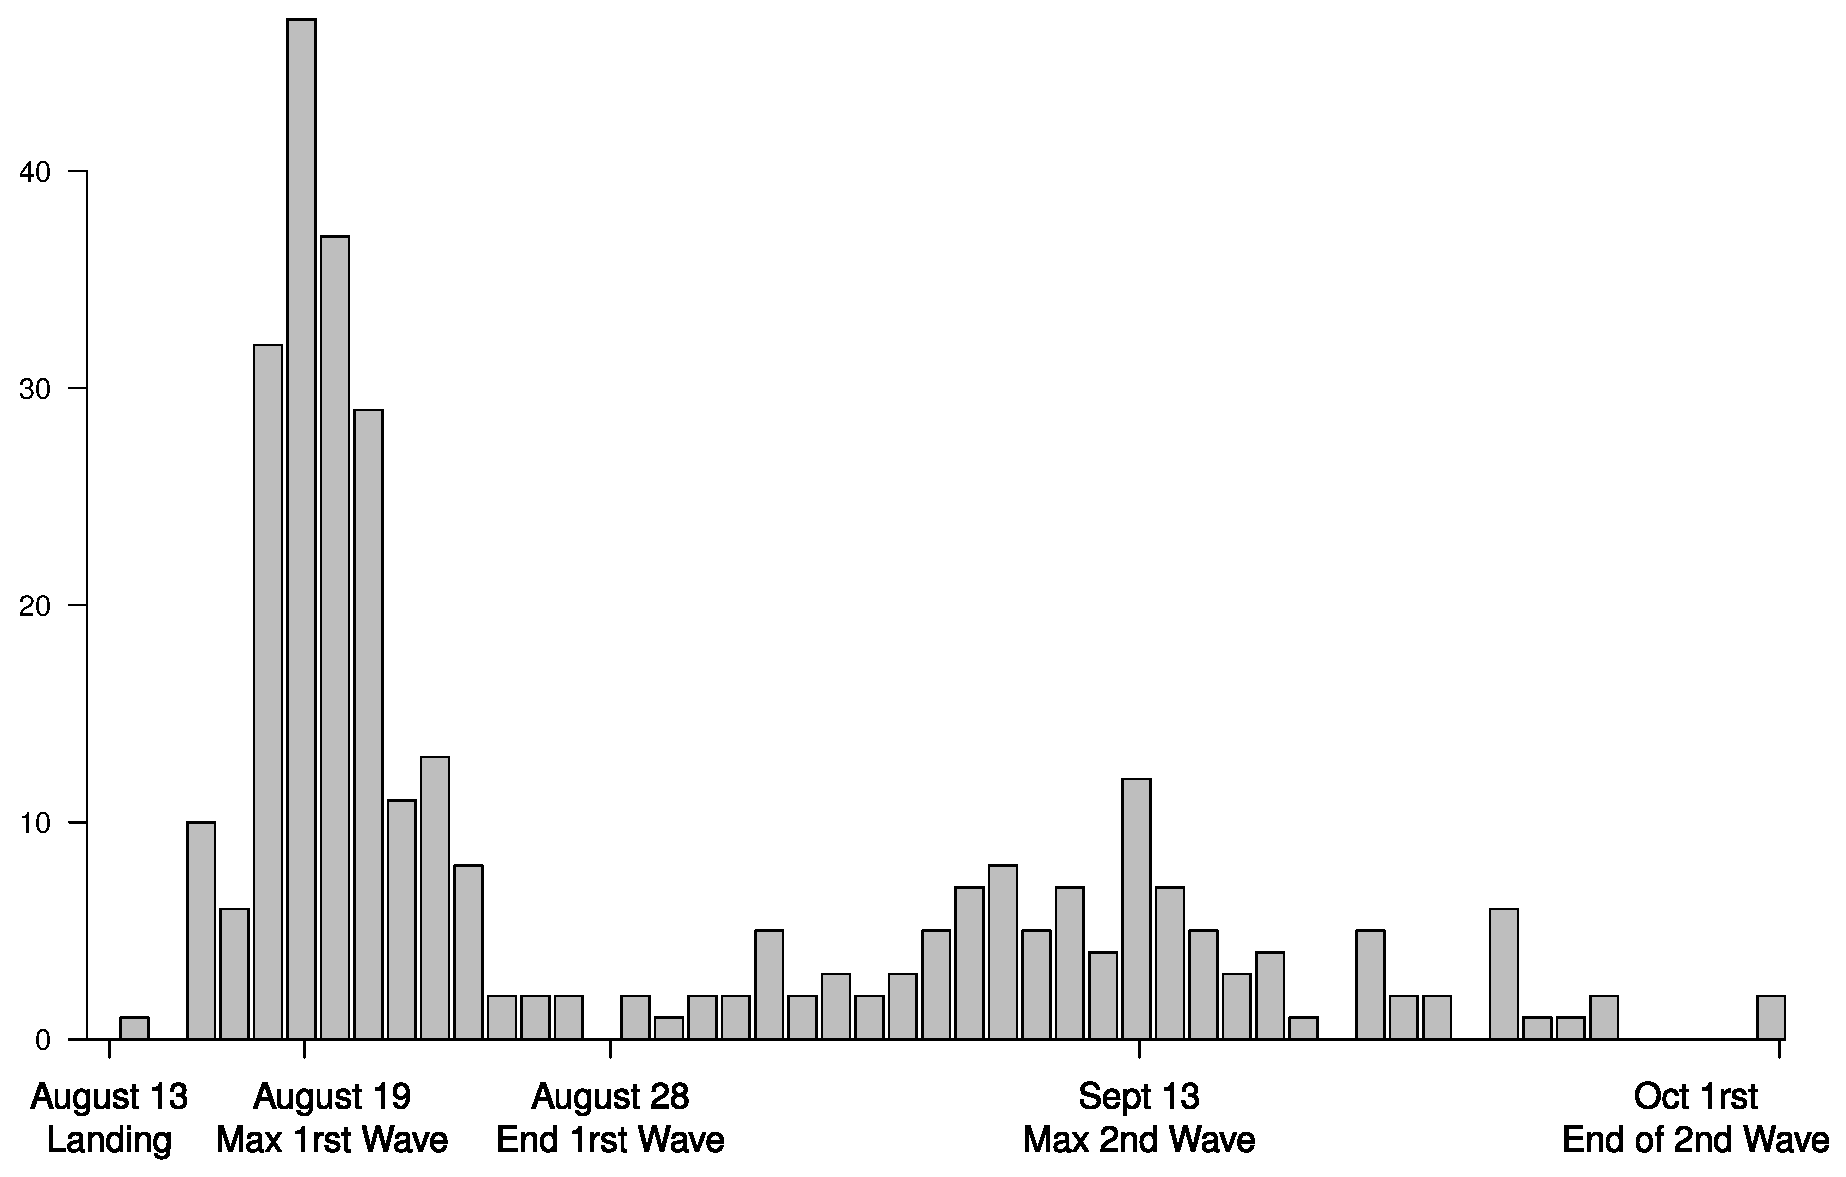
\includegraphics[width=0.7\linewidth]{texte/tdc/graph/data.eps}
\caption{Geographical position of Tristan da Cunha and incidence time series}
\label{fig:tdc}
\end{center}
\end{figure}


\section{Hypothesis Test}

Our aim was to explain the unusual influenza epidemic that occurred on
a small South-Atlantic island, named Tristan da Cunha, in 1971, 3
years after the emergence of new influenza A subtype H3N2. H3N2 was
introduced by a ship returning from Cape-Town that landed five
islanders on Tristan da Cunha. After the arrival of the ship an
influenza epidemic occurred over 50 days. But after three weeks of
propagation, while the epidemic was declining, some islanders
developed second attacks and a second peak of new cases was recorded
(see Figure \ref{fig:tdc}). Among the 284 islanders, 273 (96\%)
experienced at least one attack and 92 (32\%) experienced two attacks
(see \citet{Mantle1973} and \textsl{Material and Methods}).

Among all the explanations proposed to explain this two-wave epidemic,
\citet{Mantle1973} concluded that the hypothesis of reinfection by the
same viral agent was the only possible. However, they were unable to
determine if antigenic change in the virus have occurred, allowing for
second infection, or if some patients did not acquire an efficient
immune protection and were reinfected by other patients.
%
% (il y a aussi l'hyp de reinfection intra-hote)
%
Thus, the first biological hypothesis (subsequently referred as the
$MUT$ hypothesis) assumes that virus mutated within infected hosts
during the first epidemic-wave leading to the emergence of a new
antigenically drifted variant. However given that it normally takes
between 2 and 8 years at the scale of the global human population for
a new variant to acquire significant antigenic changes
\citep{Smith2004,Koelle2006} and since second attacks occurred only
three weeks after the beginning of the epidemic in a population of 284
individuals, we can reasonably assume that if a new variant emerged
during the first wave it had to happen within a single infected host.
The second biological hypothesis (subsequently referred as the $MI$
hypothesis) assumes that following recovery from infection some hosts
acquire a long-term protective immunity against reinfection whereas
some other become again fully susceptible to the virus. This
assumption was previously introduced by \citet{Mathews2007}. The third
hypothesis (subsequently referred as the $PP$ hypothesis) was
previously introduced by \citet{Gomes2004} and assumes that following
recovery from infection all hosts develop an immune response that is
not fully protective while reducing the risk of reinfection.

These 3 hypothesis have been translated into 3 different mathematical
models (see Figure \ref{fig:models_tdc} and \textsl{Materials and
  Methods}). Model parameters and their biological interpretation are
given in table \ref{tab1}. We used the stochastic framework for
running these 3 models. Parameter inference and model selection were
achieved through the plug-and-play framework proposed by
\citet{Ionides2006}. This frequentist approach converges to the maximum
likelihood parameter set estimate for each model and allows therefore
to compute the Akaike information criteria to select the model that
best explain the data (see \textsl{Material and Methods}).

\begin{center}
\begin{table}[htdp]
  \begin{footnotesize}
    \begin{tabular}{|l|l|c|c|c|}
      \hline
      Symbol & Description & $MUT$ & $MI$ & $PP$\\ \hline
      $R_{0}$ & basic reproductive number & 10.41 & 8.01 & 5.26 \\ \hline 
      $1/e$ & mean latent period (days) & 2.42 & 1.96 & 1.51 \\ \hline
      $1/v$ & mean infective period (days) & 1.20 & 1.39 & 0.87\\ \hline
      $1/g$ & mean temporary removed period (days) & 2.77 & 11.90 & 5.71\\ \hline
      $\alpha$ & probability to develop long-term immunity after infection & - & 0.48 &- \\ \hline
      1-$\sigma$ & partial protection induced by a first attack &0.83 &- & 0.78 \\ \hline
      $\rho$ & reporting rate for observation & 0.68 & 0.69 & 0.65 \\ \hline
      $T_{mut}$ & time of introduction of the new variant & $23^{rd}$ august &-&-\\ \hline
      $\mathcal{L}(\theta_{MLE})$ & Log-likelihood for each model &-130.03 & -106.13 & -124.11 \\ \hline
      $AIC_{c}$ & Akaike information criteria &279.41 & 231.61 & 267.57\\ \hline
    \end{tabular}
  \end{footnotesize}
\caption{Parameter description, maximum likelihood estimates and Akaike information criteria for each model}
\label{tab1}
\end{table}%
\end{center}

\begin{figure}
\begin{center}
\caption*{a) Mutation model ($MUT$)}
\label{MUT}
\begin{tikzpicture}[node distance=3cm, auto,>=latex', thick]
    %\path[use as bounding box] (-1,0) rectangle (10,-2);
    \path[->] node [expo] (sain) {S}
     	    node [erlang, right of=sain] (expose) {E1}
    node [erlang, right of=expose] (infecte) {I1}
    node [expo, right of=infecte] (immunise) {R1}
     (sain) edge node {$\beta$} (expose)
     (expose) edge node[name=e] {$e$}(infecte)
     (infecte) edge node{$v$}(immunise);
  
   \path[->]  node [erlang_2, below of=e] (infecte_2) {I2};
   %\path[->]  (infecte) edge[dashed] node{$\mathds{1}_{T_{mut}}$}(infecte_2);
    
         \path[->] node [erlang_2, right of=infecte_2] (expose_2) {E2}
    node [expo_2, left of=infecte_2] (immunise_2) {R2}
    
     
     (sain) edge node[near start,below] {$\beta$} (expose_2)   
     (infecte) edge node{$v$}(immunise) 	
     (immunise) edge node[near start] {$\sigma\beta$} (expose_2)
     (expose_2) edge node{$e$}(infecte_2)
     
     (infecte_2) edge node{$v$}(immunise_2);

\end{tikzpicture}


\vspace{0.5cm}
\caption*{b) Multiple-Infection model ($MI$)}
\begin{tikzpicture}[node distance=2cm, auto,>=latex', thick]

    % We need to set at bounding box first. Otherwise the diagram
    % will change position for each frame.
   % \path[use as bounding box] (-1,0) rectangle (10,-2);
     \node [expo] (sain) {S};
     	    \node [erlang, right of=sain] (expose) {E};
    \node [erlang, right of=expose] (infecte) {I};
    \node [erlang, right of=infecte] (immunise) {R};
    \node [expo, right of=immunise] (longue) {L};

% Once the nodes are placed, connecting them is easy. 
    \draw [->] (sain) -- node {$\beta$} (expose);
    \draw [->] (expose) -- node{$e$}(infecte);
    \draw [->] (infecte) -- node{$v$}(immunise);
    \draw [->] (immunise) -- node{$\alpha g$}(longue);
    \draw[->](immunise) -- +(0,1) -| node[near start,above] {$(1-\alpha)g$} (sain);
    
\end{tikzpicture}
%\label{MI}
\vspace{0.5cm}
\caption*{c) Partial-Protection model ($PP$)}
\begin{tikzpicture}[node distance=2cm, auto,>=latex', thick]
    % We need to set at bounding box first. Otherwise the diagram
    % will change position for each frame.
   % \path[use as bounding box] (-1,0) rectangle (10,-2);
     \node [expo] (sain) {S};
     	    \node [erlang, right of=sain] (expose) {E};
    \node [erlang, right of=expose] (infecte) {I};
    \node [erlang, right of=infecte] (immunise) {R};
    \node [expo, right of=immunise] (longue) {L};

% Once the nodes are placed, connecting them is easy. 
    \draw [->] (sain) -- node {$\beta$} (expose);
    \draw [->] (expose) -- node{$e$}(infecte);
    \draw [->] (infecte) -- node{$v$}(immunise);
    \draw [->] (immunise) -- node{$g$}(longue);
    \draw[->](longue) -- +(0,1) -| node[near start,above] {$\sigma\beta$} (expose);
    
\end{tikzpicture}
%\label{PP}
\end{center}
\caption{Three models with three different biological
  mechanisms. Square boxes stand for Erlang distribution for the
  residence durations into states $E$,$I$ and $R$ (shape $k=2$ and
  mean values $1/e$,$1/v$ and $1/g$). Circle boxes stand for simple
  exponential durations. Parameter description can be found in table
  \ref{tab1}.}
\label{fig:models_tdc}
\end{figure}


\section{Results}

Maximum likelihood estimate for the parameter set of each model is
presented in table \ref{tab1}. Estimates vary somewhat between models
and are characterized by a high $R_{0}$ ($> 5$), an infective period
of about one day and a latent period of about two days. Regarding the
$MI$ model estimate of $\alpha$ shows that in proportion about half of
the infected hosts did not develop a long-term protective immunity
after the first exposure. In contrast, for the $MUT$ and $PP$ models
estimates of the level of cross-protection conferred by the first
exposure is around 80\%. This discrepancy is however balanced by a
shorter temporary removed duration allowing hosts to be potentially
faster reinfected in both $PP$ and $MUT$ models than in the $MI$
model. The reporting rate ($\rho$) \textit{i.e.} the proportion of the
total cases that were reported, is estimated for all three models
around 70\%, which is under the minimal value of 85\% due to data
uncertainties (see \textsl{Material and Methods}). These parameter set
estimates are confirmed by the bayesian approach of \citet{Toni2009}
(see the supplementary document).

Figure \ref{res1} compares the average prediction of each model with
maximum likelihood parameter estimates. Whereas all three models
easily fit the first wave only the $MI$ model can capture the second
wave. This observation is statistically confirmed by the Akaike
information criteria which shows that the $MI$ model best explains the
data (see table \ref{tab1}). We also note that the $MUT$ model is the
least likelihood.

In order to understand why neither $PP$ nor $MUT$ models succeed to
capture the second wave epidemic (figure \ref{res1}) we calculated the
evolution of the extinction probability. Thus for all three models we
computed at each point in time the proportion of extinct simulations
over 100000 stochastic realizations. Results are shown on figure
\ref{res1} and point out the role of demographic
stochasticity. Indeed, whereas the extinction probability increases
rapidly at the end of the first wave for both $PP$ and $MUT$ models,
the $MI$ model appears to be much more robust to stochastic
extinctions during the inter-wave period. This conclusion is all the
more surprising that estimate of the temporary removed duration
($1/g$) is well above for the $MI$ model than for the other two.
Regarding the $MUT$ model, the sudden increase of the extinction
probability corresponds to a high risk of failed invasion for the
newly emerging variant in the population \citep{Lloyd-Smith2005}. The
case of the $PP$ model is more complicated. Previous analysis of a
similar but deterministic model \citep{Gomes2004,Gomes2005} have
revealed that dynamics are depending on a reinfection parameter
$\sigma R_{0}$. When this parameter is well above a reinfection
threshold \textit{i.e.} $\sigma R_{0}>1$, reinfection becomes
self-sustained and dynamics are $SIS$-like whereas below this
threshold primary infection dominates and leads to $SIR$-like
dynamics. Estimate for our stochastic $PP$ model gives $\sigma
R_{0}=1.3$ and indicates a critical dynamics: the reinfection
parameter needs to be sufficiently high to reduce stochastic
extinctions during the inter-wave period but in the same time it must
be sufficiently low to avoid sustained reinfection leading to more
than two epidemic waves. In other words the observed epidemic
extinction after the second wave decreases the reinfection parameter
and therefore increases the inter-wave extinction probability.

\begin{figure}
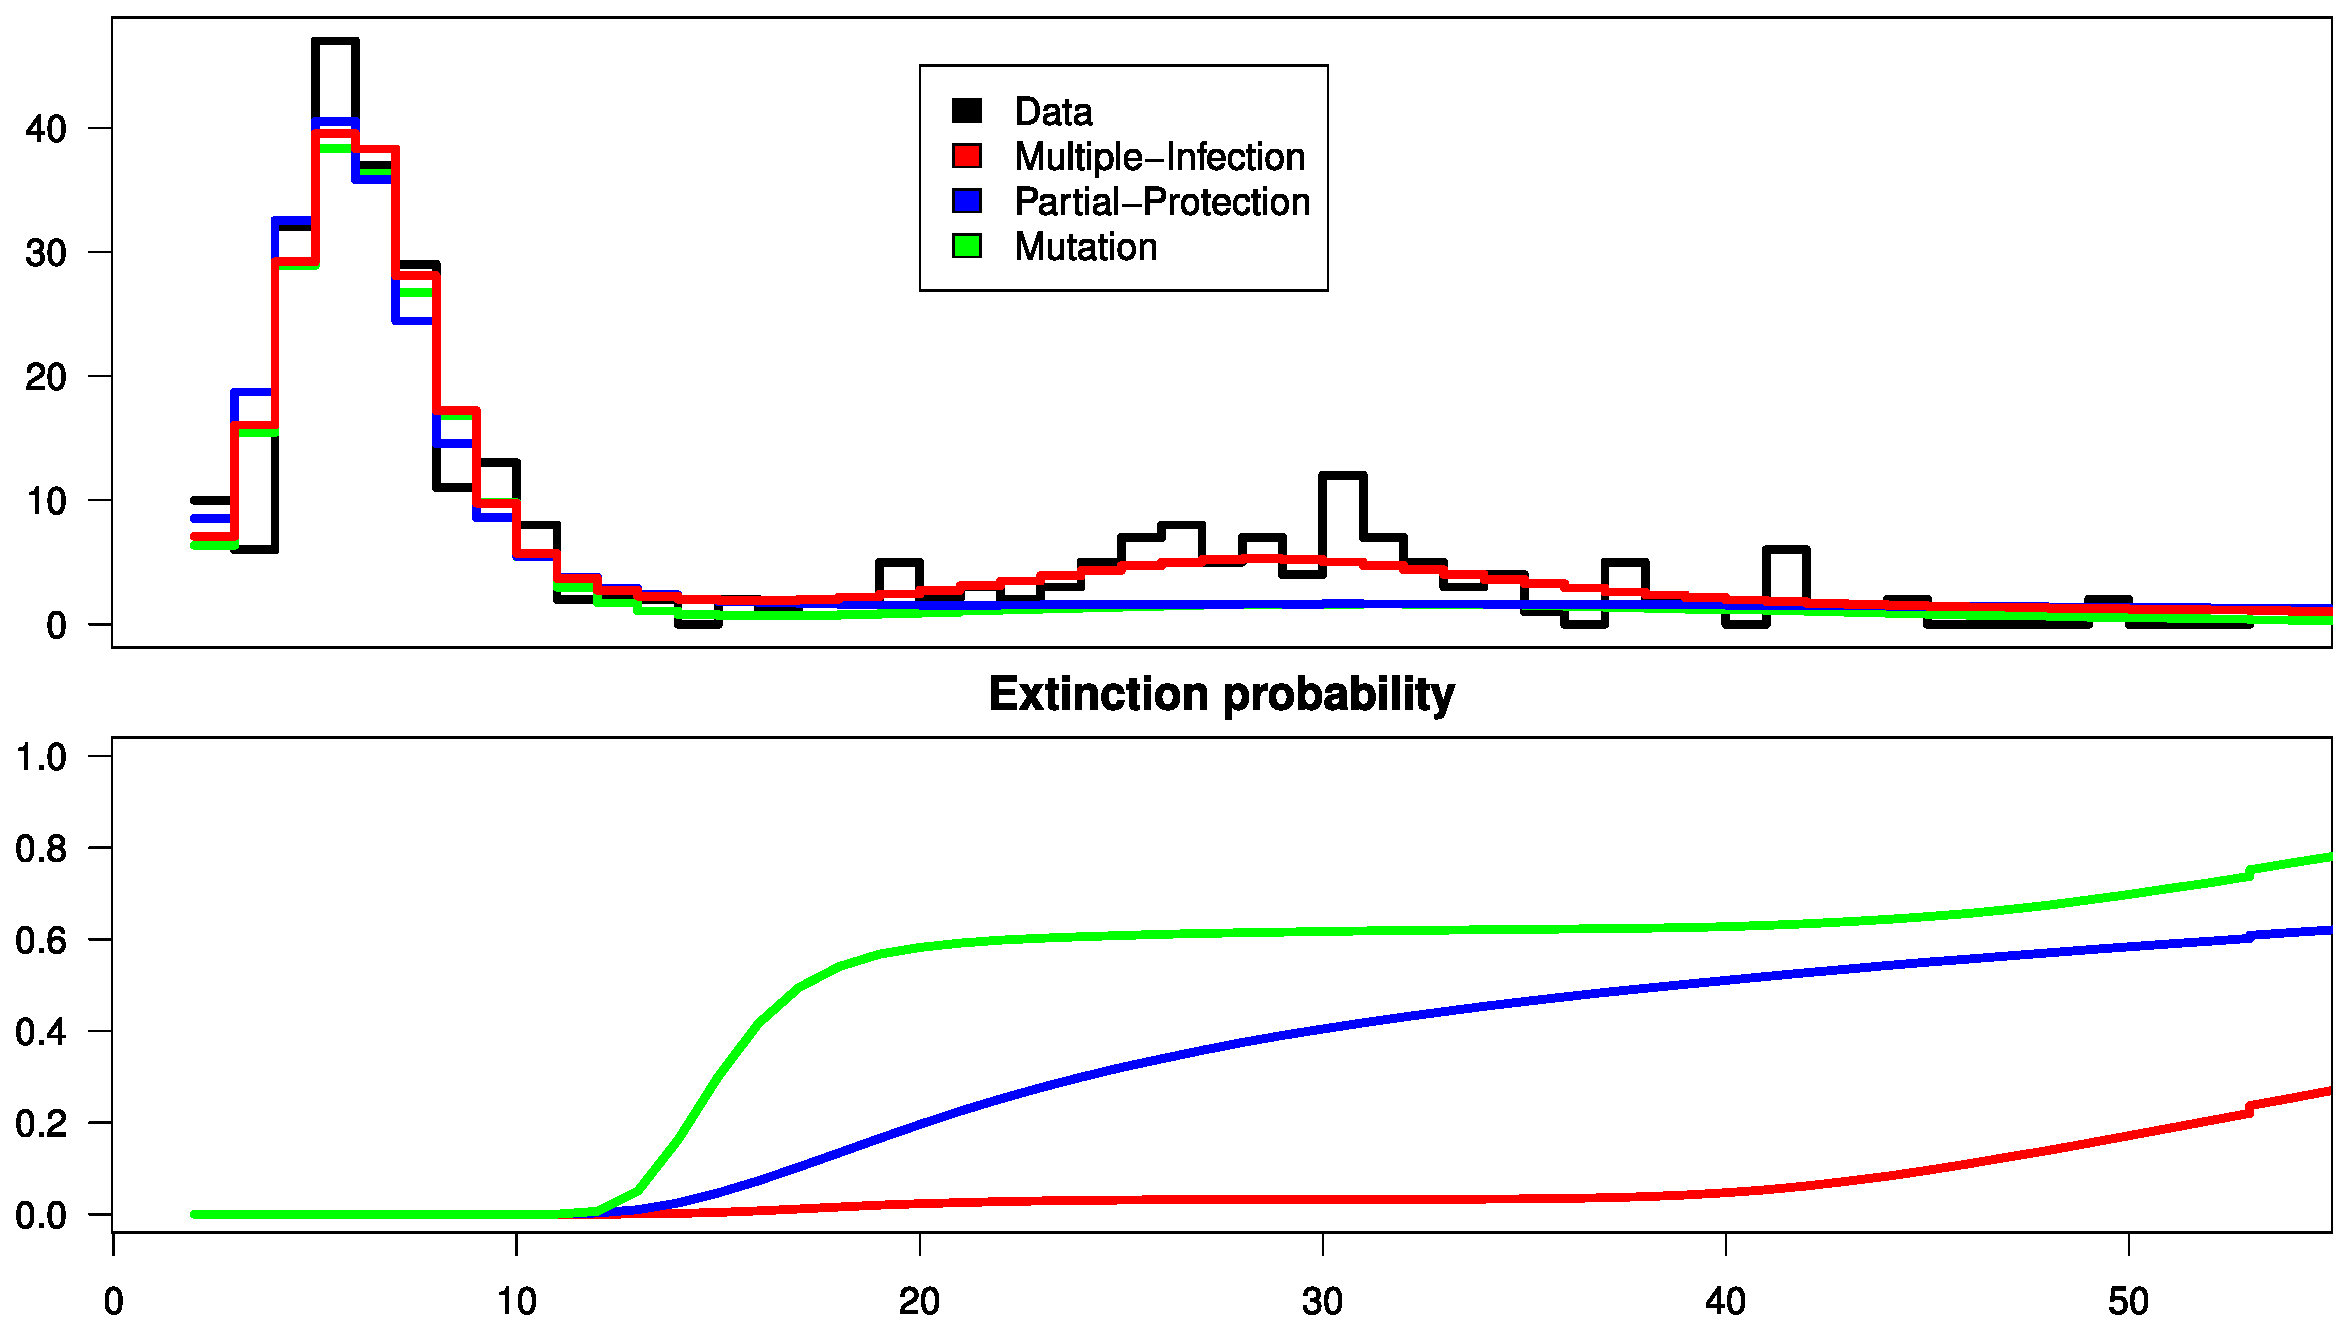
\includegraphics[width=0.9\linewidth]{texte/tdc/graph/res_et_extinction.eps}
\caption{Average prediction of each model with maximum likelihood parameter estimates}
\label{res1}
\end{figure}

\section{Discussion}

In this study we propose to use simple mathematical models to
disentangle between three biological mechanisms for explaining a
two-wave epidemic of influenza A/H3N2 on the island of Tristan da
Cunha in 1971. Following a model selection based on a rigorous
statistical framework \citep{Ionides2006}, we show that the most
likely explanation is that only 50\% of the patients developed a
long-lasting protection against the virus after the first attack
whereas unprotected hosts developed illness following re-exposure to
the same virus and initiated the second epidemic wave.

In a previous study \citet{Mathews2007} fitted a flexible model
(similar to our $MI$ model) on the same data set using a deterministic
framework. Their parameter estimate was achieved via MCMC but after
comparison of their mean estimate with our maximum likelihood estimate
we find very close values except for the mean serial interval
(infectious plus latent period), which is slightly greater in our
study (2.24 vs. 3.4 days). We think that this discrepancy is mainly
attributable to the incorporation of demographic stochasticity in our
approach: by fitting a deterministic model \citet{Mathews2007} neglect
the probability of stochastic extinction and implicitly underestimate
the duration of the serial interval which plays a significant role
during the inter-wave period. This remark emphasizes the need to use
stochastic simulations for parameter inference whenever the population
is low and/or demographic stochasticity is expected to play a
significant role \citep{Lloyd-Smith2005}.

Our estimates for the mean latent and infective periods of the $MI$
model are close to previous published estimates \citep{Cauchemez2004}
whereas the high value of the basic reproductive number is somewhat
unexpected for influenza virus since $R_{0}$ is usually estimated
around 2 \citep{Lessler2007}. However the rapid spreading of the virus
(the first peak was reached after 6 days only) as well as the
unusually high attack rate, which is typical of small isolated
communities \citep{Brown1966}, and the exceptional contact
configuration of the population of Tristan da Cunha
\citep{Samuels1963,Shibli1971} give support to such a high $R_{0}$
value \citep{Mathews2009}. Moreover, as we point out in the
\textsl{Material and Methods}, the single influenza virus most
islanders were exposed to before the epidemic of 1971 was a polyvalent
influenza vaccine dating from 1961 \citep{Tyrrell1967}. This vaccine
contained only an H2N2 strain and a B strain and it is unlikely to
have conferred protection against H3N2
\citep{Brown1969a,Brown1969b}. The high susceptibility of the
islanders to influenza contrasts with existing prior-immunity in
uninsulated communities and could contribute to the high estimated
value of $R_{0}$ \citep{McVernon2007,McCaw2009}.

The hypothesis of homogeneous mixing underlying the infection process
in our models may seem questionable even for the small population of
Tristan da Cunha \citep{Becker1983}. However it is a reasonable
assumption since topographical or sociological grouping
\citep{Shibli1971} are not expected to play a significant role on the
progress of the epidemic \citep{Hammond1971}.

From a more immunological stand point, human immune response to a
novel antigen/virus remains poorly understood in the case of influenza
although it is of first importance for managing a new pandemic
\citep{Doherty2006}. This response varies among individuals and
previous works have argued that such variability could depend on two
factors: the way the antigen/virus is introduced into the organism and
the immune history of the infected host. Indeed, it is commonly
admitted that a single natural infection by an influenza strain
confers life-long immunity against this strain whereas two vaccine
injections may usually be necessary to guarantee protection.
% (ref?)
%
Regarding the immune history, hosts with prior exposure and
pre-existent antibodies to several influenza strains have usually a
better response to vaccination \citep{Brown1969a} although it has also
been reported that these hosts could suffer from an original antigenic
sin \textit{i.e.} infection by a new influenza variant induces a
strong recall of antibodies against previously encountered antigens
but a weak immune response against the novel antigens \citep{Kim2009}.

Nevertheless the original antigenic sin mechanism may not have been
involved in the lack of immune response for 50\% of the population of
Tristan da Cunha since the level of prior-exposure to influenza virus
was unusually low in this population. Moreover, previous studies of
isolated naive communities have shown evidences for high specific
immune response following natural infection
\citep{Brown1966,Brown1969a,Brown1969b}.
%(confirmer, par ailleurs lors d'un antigenic sin on peut quand me gur
%de la premie attaque?).

Generally, isolated communities are expected to be less exposed, and
then more susceptible, to many diseases otherwise commonly encountered
in uninsulated populations. This obvious fact was confirmed for the
population of Tristan da Cunha after its evacuation due to a volcano
eruption in 1961. It was then reported that most adults suffered from
children diseases during their 2-year stay in Great-Britain
\citep{Tyrrell1967}. Thus, regarding influenza, the naive population
of Tristan da Cunha can reasonably be considered immunologically
closer to child than to adults of uninsulated communities before the
A/H3N2 epidemic of 1971.

Among the studies that have reported explicit cases of reinfection
during pandemic or inter-pandemic seasons, some presented significant
differences between children and adults the former being less
protected than the latter \citep{McVernon2007}. For example,
\citet{FOX1982a,FOX1982b} reported cases of reinfection by H3N2 during
the period of 1975-1979 in Seattle families. Their serological
analysis revealed that in those under (resp. above) age 20 years 36\%
(resp. 24\%) were reinfected, 75\% (resp. 17\%) of whom developed
illness. By comparing the HI titers of the two groups they found that
high titers $(\geqslant 1:40)$ were conferring protection against
illness only in the above 20 year age group.
% only the adults with low titers (<1:40) developed illness after reinfection whereas in the under 20 year age group high titers conferred no protection against illness.

Whereas the study of \citeauthor{FOX1982a} was conduced during an
inter-pandemic episode and over a much larger time scale than in our
case-study, the reported infection pattern of the under 20 year age
group seems very comparable to the one observed in the population of
Tristan da Cunha.

%This last remark calls for careful surveillance of naive populations such as the younger during pandemic episodes since even after a first attack these populations could be reinfected and keep the spread of the epidemic. 


On the other hand, even if it is not straightforward to compare
vaccination with natural infection, vaccination experiments during
past influenza pandemic tend also to support the idea that multiple
infections in immunologically naive hosts are needed before mounting a
protective immune response. For instance, whereas a single injection
of H1N1 vaccine was giving as good response as two injections prior to
1957, the advent of H2N2 pandemic in 1957 changed the situation since
two injections became necessary to confer protection
\citep{HOLLAND1958}.  The re-introduction of H1N1 in 1977-1978 also
offers an interesting case study as two injections of vaccine were
more effective than a single injection for children and young adults
whereas less difference was detected in hosts infected with H1N1 at
least 20 years earlier \citep{Nicholson1979}.


In conclusion, the importance of the present analysis is to highlight
the influence of reinfection in an influenza epidemic that occurred in
the unusually well-documented population of Tristan da Cunha. Our
results suggest that some people need multiple exposures to the virus
before developing a sufficiently immunological response and a
protective immunological memory. These historical data alone cannot
prove the importance of reinfection and immunological maturation in
influenza epidemics in a naive population nevertheless our findings
suggest that it may play a non-negligible role and call for careful
surveillance of naive populations, such as the youths, during pandemic
episodes since even after a first attack these populations could be
reinfected and keep the spread of the virus.


\section{Materials and Methods}

\subsection{Data}

Tristan da Cunha is a volcanic island in the South Atlantic Ocean. It
has been inhabited since the $19^{th}$ century and in 1971, the 284
islanders and 20 expatriates were living in the single village of the
island: Edinburgh of the Seven Seas (\citet{Samuels1963}, Figure
\ref{fig:tdc}). Whereas the internal contacts were typical of
well-knit village communities, contacts with the outside world were
infrequent and mostly due to fishing vessels that occasionally were
taking passengers to or from the island. These ships were often the
cause of introduction of new diseases on the population. Focusing on
influenza, several serological analysis between 1955 and 1963 provide
important insight into the immune status of the 284 islanders before
1971. Following an epidemic of H1N1 in 1954 during which most of the
islanders were infected, antibodies to older influenza A and B types
were detected in islanders over 20 years of age
\citep{Taylor-Robinson1963}. In 1961 when the volcano erupted the
island was evacuated to Britain via Cape-Town and the islanders were
given a polyvalent influenza vaccine that contained an H2N2 strain and
a recent B strain. Antibody studies showed a good response to this
inoculation \citep{Tyrrell1967}. Since the population returned to
Tristan da Cunha in 1963, no influenza epidemic has been reported. In
this context of a small population with weak and homogenous immune
repertoire against influenza virus, an unusual epidemic occurred in
1971, 3 years after the emergence of new subtype H3N2.

On august $13^{th}$, a ship returning from Cape-Town landed five
islanders on Tristan da Cunha. Three of them developed acute
respiratory disease during the 8-day voyage and the other two
presented similar symptoms immediately after landing. Various family
gatherings welcomed their disembarkation and in the next day epidemic
started to spread rapidly throughout the whole island
population. After three weeks of propagation, while the epidemic was
declining, some islanders developed second attacks and a second peak
of new cases was recorded. The epidemic fade out after this second
wave and lasted a total of fifty days.

Among the 284 islanders, 273 (96\%) experienced at least one attack
and 92 (32\%, mainly adults) experienced two attacks. Only few
individuals experienced their single attack during the second epidemic
wave. Unfortunately, only 312 of the 365 attacks (85\%) are known
within a single day accuracy and constitute the data set
\citep{Mathews2007}. These uncertainties can nevertheless be managed
since the statistical framework of \citet{Ionides2006} allows for
measurement errors. A precise description of the clinical features of
the illness as well as a review of the secondary infections were
provided by \citet{Mantle1973}. They reported that 85\% of the first
attacks were moderate or severe and this proportion decreased to 50\%
for the second attacks. However, they noted that 21 individuals
experienced two severe attacks. Serological analysis of infected
individuals demonstrated a high level of antibody against H3N2, a
subtype the population was never exposed to. Moreover, this high level
was detectable in individuals infected only during the first or the
second epidemic wave, attesting that the virus was circulating
throughout the epidemic. Unfortunately, no virological analysis were
conducted to show whether first and second attacks were due to
antigenically differing strains of H3N2.

\subsection{Models}

We model the three hypotheses via three simple mechanistic models
(Figure \ref{fig:models_tdc}). All the models use the same infection
process: after exposure to influenza virus susceptible hosts ($S$)
pass through a latent state ($E$) before becoming infectious
($I$). Infectious hosts enter the removed state ($R$) when they are
temporary unable to participate to the epidemic spreading: this may be
due to quarantine in bed or to temporary full-immunity because of
cell-mediated protection. Time spent in the $E$,$I$ and $R$ classes
follows an Erlang distribution with shape equal to 2 allowing for a
larger, more realistic, variance than the exponential
distribution. Note also that while in class $R$ hosts are protected
against reinfection.
 
The first model corresponds to the emergence of a new variant by
Mutation (labeled $MUT$). It is implemented by a history-based
2-strains model. The new variant is introduced at a single point of
time when an infectious host with strain 1 becomes infectious with
strain 2 (for simplicity, co-infection is not allowed). Both strains
are supposed to have the same transmissibility and to cross-react
\textit{i.e.} following infection by a single strain, as hosts leave
the removed class $R$ to enter the class $L$ they benefit a reduction
of susceptibility $\sigma$ against infection by the other strain.

The second model corresponds to the assumption that some hosts need
Multiple Infection before acquiring a long-term immunity (labeled
$MI$). When leaving the temporary removed state ($R$), each host has a
probability $\alpha$ to develop a long-term protection against
reinfection entering class $L$, otherwise host becomes again fully
susceptible to the virus and re-enter class $S$.

The third model corresponds to the assumption that long-term immunity
is always developed after infection while only Partially Protective
against reinfection (labeled $PP$). When leaving the temporary removed
state ($R$), each host enters the long-term immunity class $L$ and
benefit a reduction of susceptibility $\sigma$ against reinfection.

\subsection{Simulation and model selection} 


Given the small population of Tristan da Cunha demographic
stochasticity is expected to play a significant role in the epidemic
dynamics, especially during the inter-wave period when the number of
infected hosts is low and epidemic fade-out is likely to happen. We
therefore used the stochastic framework of continuous-time Markov
processes that naturally allows to take demographic stochasticity into
account.

Identification and model comparison have been performed with a
plug-and-play framework perfectly adapted to nonlinear stochastic
models \citep{Ionides2006,Breto2009,Toni2009}. In this paper we choose
to use the frequentist framework of iterated filtering
\citep{Ionides2006,King2008} due to its computational efficiency. In
addition we have confirmed the parameter inference for all models via
the bayesian approach of \citet{Toni2009}.

Numerical simulations were performed using the exact algorithm
provided by \citet{Gillespie1977}. Model predicted incidence is
computed by counting the daily number of new hosts entering the
infectious class $I$. Since the data set reports only 85\% of the
total number of attacks and in order to take into account measurement
errors, the observation process must also be modeled. We use a Poisson
process observation whose reporting rate parameter ($\rho$) is also
inferred \citep{Ionides2006,Breto2009}. Thus, we fitted each model to
infer the parameter set that maximizes the likelihood. Convergence to
the maximum likelihood was checked by computing profile likelihood
(see the supplementary document). These parameter sets were used to
simulate the average prediction of each model over 100000 runs and we
computed the corresponding likelihood. Finally we used the Akaike
information criteria to select the model that best explain the data:
$AIC_c=-2\mathcal{L}(\theta_{MLE})+2k+\frac{2k(k+1)}{n-k-1}$ where $k$
is the number of parameters and $n$ is the number of observations.



%%% Local Variables: 
%%% mode: latex
%%% TeX-master: "../../phD"
%%% End: 
